\begin{exercise}{La torpille}{1}{Sup}
{Cinématique}{lelay}

Un navire $N$ est animé d'un mouvement rectiligne uniforme de vitesse $\vec{v}$ le long d'une droite $D$. Un sous marin immobile $S$ tire une torpille $T$ de vitesse $\vec{u}$ au moment à l'angle $(\vec{SN}, \vec{v})$ vaut $\alpha$.

\begin{center}
    \begin{tikzpicture}
    
    % Le navire
    \node (N) at (-4,0) {};
    \filldraw[black,thick] (N) circle [radius=3pt] ;
    \draw (N) node[above=2pt] {$N$};
    
    % La trajectoire
    \draw[gray, thick] (-5,0) -- (2,0);
    \draw (1.5,0) node[above=1pt] {$D$};
    
    % Le vecteur vitesse
    \node (v) at (-2,0) {};
    \draw[black, thick, ->] (N) -- (v);
    \path (N) -- coordinate[midway](labelv) (v);
    \draw (labelv) node[above=2pt] {$\vec{v}$};
    
    % Le sous marin
    \node (S) at (0,-3) {};
    \filldraw[black,thick] (S) circle [radius=3pt] ;
    \draw (S) node[below=2pt] {$S$};
    
    % La droite
    \draw[gray, thick, dotted] (S) -- (N);
    \draw[black] (-2.5,0) arc (0:-36.9:1.5);
    \draw (-2.5,-0.5) node[anchor=west] {$\alpha$};
    
    % Interception des trajectoires (cible)
    \node (C) at (-1,0) {};
    % \filldraw[black,thick] (C) circle [radius=3pt] ;
    % \draw (C) node[above=2pt] {$C$};
    
    % Trajectoire de la torpille
    \draw[gray, thick, dotted] (S) -- (C);
    
    % Position de la torpille
    \path (S) -- coordinate[midway](T) (C);
    \filldraw[black,thick] (T) circle [radius=2pt] ;
    \draw (T) node[right=2pt] {$T$};
    
    % Vecter vitesse de la torpille
    \path (T) -- coordinate[midway](u) (C);
    \draw[black, thick, ->] (T) -- (u);
    \path (T) -- coordinate[midway](labelu) (u);
    \draw (labelu) node[above right=1.5pt] {$\vec{u}$};
    
    \draw[black] (T) arc (105:143:1.5);
    \draw (-1.4,-1.5) node[anchor=west] {$\theta$};
    
    
    \end{tikzpicture}
\end{center}

\begin{questions}
    \questioncours Rappeler la définition d'un référentiel et d'un repère. Dans quel référentiel se place-t-on ici ?
    \question Commenter le schéma et identifier les cas limites.
    \question Quelle doit être la valeur de l'angle de tir $\theta = (\vec{SN}, \vec{u})$ pour que la torpille atteigne sa cible ?
    \question On souhaite que la torpille atteigne le navire en un temps minimum. Pour quelle valeur de $\alpha$ convient-il de tirer ? Calculer l'angle de tir correspondant. Interpréter ces résultats dans les limites $ u \gg v$ et $u \ll v$
\end{questions}

\end{exercise}

\begin{solution}


\begin{questions}
    \questioncours Rappeler la définition d'un référentiel et d'un repère. Dans quel référentiel se place-t-on ici ?
    \question L'idée est de réfléchir physiquement. Plein de choses à dire en regardant le dessin, par exemple :
    \begin{itemize}
        \item $u \gg v$ : $\theta \rightarrow 0$
        \item $v \gg u$ : impossible
        \item Si $\alpha \geq \pi/2$, on doit avoir $u \geq v$
        \item Si $\alpha = \pi/2$ et $u = v$, $\theta = \pi/4$
    \end{itemize}
    
    \question 2 possibilités :
    \begin{itemize}
        \item Utiliser la distance MC, M étant le projeté orthogonal du point de croisement des trajectoires (C) sur la droite reliant S à N. la distance MC est alros $MC = d = ut \sin \theta = v t \sin \alpha$ avec $t$ le temps de trajet de la torpille
        \item Partir directement de la loi des sinus : $\sin \alpha / uT = \sin \theta / vT$
    \end{itemize}
    À la fin on doit trouver $u \sin \theta = v \sin \alpha$
    
\begin{center}
    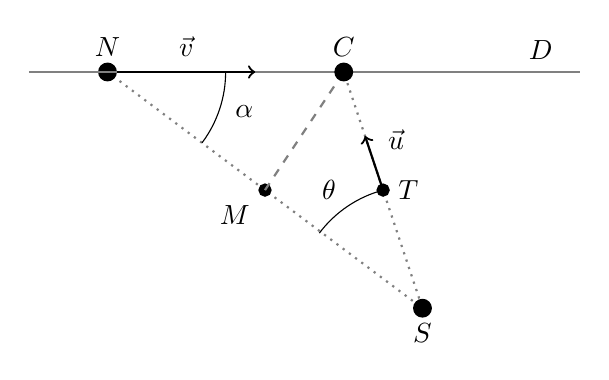
\begin{tikzpicture}
    
    % Le navire
    \node (N) at (-4,0) {};
    \filldraw[black,thick] (N) circle [radius=3pt] ;
    \draw (N) node[above=2pt] {$N$};
    
    % La trajectoire
    \draw[gray, thick] (-5,0) -- (2,0);
    \draw (1.5,0) node[above=1pt] {$D$};
    
    % Le vecteur vitesse
    \node (v) at (-2,0) {};
    \draw[black, thick, ->] (N) -- (v);
    \path (N) -- coordinate[midway](labelv) (v);
    \draw (labelv) node[above=2pt] {$\vec{v}$};
    
    % Le sous marin
    \node (S) at (0,-3) {};
    \filldraw[black,thick] (S) circle [radius=3pt] ;
    \draw (S) node[below=2pt] {$S$};
    
    % La droite
    \draw[gray, thick, dotted] (S) -- (N);
    \draw[black] (-2.5,0) arc (0:-36.9:1.5);
    \draw (-2.5,-0.5) node[anchor=west] {$\alpha$};
    
    % Interception des trajectoires (cible)
    \node (C) at (-1,0) {};
    \filldraw[black,thick] (C) circle [radius=3pt] ;
    \draw (C) node[above=2pt] {$C$};
    
    % Trajectoire de la torpille
    \draw[gray, thick, dotted] (S) -- (C);
    
    % Position de la torpille
    \path (S) -- coordinate[midway](T) (C);
    \filldraw[black,thick] (T) circle [radius=2pt] ;
    \draw (T) node[right=2pt] {$T$};
    
    % Vecter vitesse de la torpille
    \path (T) -- coordinate[midway](u) (C);
    \draw[black, thick, ->] (T) -- (u);
    \path (T) -- coordinate[midway](labelu) (u);
    \draw (labelu) node[above right=1.5pt] {$\vec{u}$};
    
    % angle theta
    \draw[black] (T) arc (105:143:1.5);
    \draw (-1.4,-1.5) node[anchor=west] {$\theta$};
    
    % Projeté orthogonal
    \path (N) -- coordinate[midway](M) (S);
    \filldraw[black,thick] (M) circle [radius=2pt] ;
    \draw (M) node[below left=2pt] {$M$};
    
    \draw[gray, thick, dashed] (M) -- (C);
    
    \end{tikzpicture}
\end{center}
    
    \question Il faut que la trejectoire de la torpille soit minimale : On frappe le navire lorsque il est a la distance minimale. On a alors $\theta = \arctan v/ u$ et $\alpha = \arctan(u / v)$
    
\begin{center}
    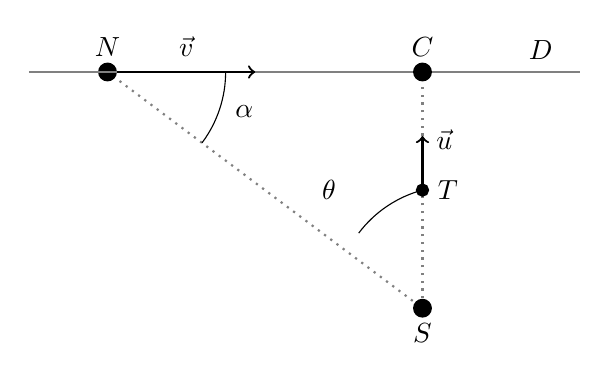
\begin{tikzpicture}
    
    % Le navire
    \node (N) at (-4,0) {};
    \filldraw[black,thick] (N) circle [radius=3pt] ;
    \draw (N) node[above=2pt] {$N$};
    
    % La trajectoire
    \draw[gray, thick] (-5,0) -- (2,0);
    \draw (1.5,0) node[above=1pt] {$D$};
    
    % Le vecteur vitesse
    \node (v) at (-2,0) {};
    \draw[black, thick, ->] (N) -- (v);
    \path (N) -- coordinate[midway](labelv) (v);
    \draw (labelv) node[above=2pt] {$\vec{v}$};
    
    % Le sous marin
    \node (S) at (0,-3) {};
    \filldraw[black,thick] (S) circle [radius=3pt] ;
    \draw (S) node[below=2pt] {$S$};
    
    % La droite
    \draw[gray, thick, dotted] (S) -- (N);
    \draw[black] (-2.5,0) arc (0:-36.9:1.5);
    \draw (-2.5,-0.5) node[anchor=west] {$\alpha$};
    
    % Interception des trajectoires (cible)
    \node (C) at (0,0) {};
    \filldraw[black,thick] (C) circle [radius=3pt] ;
    \draw (C) node[above=2pt] {$C$};
    
    % Trajectoire de la torpille
    \draw[gray, thick, dotted] (S) -- (C);
    
    % Position de la torpille
    \path (S) -- coordinate[midway](T) (C);
    \filldraw[black,thick] (T) circle [radius=2pt] ;
    \draw (T) node[right=2pt] {$T$};
    
    % Vecter vitesse de la torpille
    \path (T) -- coordinate[midway](u) (C);
    \draw[black, thick, ->] (T) -- (u);
    \path (T) -- coordinate[midway](labelu) (u);
    \draw (labelu) node[above right=1.5pt] {$\vec{u}$};
    
    % angle theta
    \draw[black] (T) arc (105:143:1.5);
    \draw (-1.4,-1.5) node[anchor=west] {$\theta$};
    
    
    \end{tikzpicture}
\end{center}
\end{questions}

\end{solution}
